\documentclass[a4paper,11pt]{article}
\usepackage{lecturenotes}
\usetikzlibrary{arrows.meta}
\lectureheader{ELE727}{3}
\begin{document}
\tableofcontents
\clearpage
\notesection{Basic Current Mirrors}
\begin{notecircuit}[american, scale=0.55, transform shape]{Basic NMOS Current Mirror}
    % Mirror M1 so its gate faces M2, as in the reference diagram.
    \node[nmos,arrowmos,xscale=-1] (M1) at (0,0) {};
    \node[nmos,arrowmos] (M2) at (2.6,1.0) {};
    \node at (0.6,-0.65) {$M_1$};
    \node at (2.0,0.35) {$M_2$};
    \node[left] at (-0.45,0) {$\dfrac{W}{L}$};
    \node[right] at (3.05,1.0) {$\dfrac{W}{L}$};
    \draw (M1.S) -- ++(0,-0.2) node[ground] {};
    \draw (M2.S) -- ++(0,-0.2) node[ground] {};

    % The reference node ties M1's drain to both gates.
    \coordinate (ref) at (M1.D |- M2.G);
    \coordinate (gate-tie) at (M1.G |- M2.G);
    \draw (M1.D) -- (ref) node[circ] {}
    -- (gate-tie) node[circ] {} -- (M2.G);
    \draw (M1.G) -- (gate-tie);

    % Reference current flows downward from V_DD.
    \draw (0,2.85) node[vcc] {$V_{DD}$}
    -- (0,2.65) to[I,l=$I_{\mathrm{REF}}$] (ref);

    % M2 sinks the analog circuit's output current.
    \node[draw,thick,align=center,font=\sffamily\bfseries,
        minimum width=1.9cm,minimum height=1.25cm,inner sep=4pt]
    (load) at (2.6,3.5) {Analog\\Circuit};
    \draw (load.south) to[short,i=$I_{\mathrm{out}}$] (M2.D);
\end{notecircuit}

To derive the relation between $I_{out}$ and $I_{ref}$, we simply use the defintion of the drain current for a transistor in saturation. It is then obvious that the currents are related through the sizing of the transistor devices:

\keyequation{Current \textit{Gain} in a Simple Current Mirror}{ I_{out} = \frac{(W/L)_2}{(W/L)_1} I_{REF}}

\notedefinition{Unit Transistor}{A unit transistor is a fixed W/L transistor used as a building block which can be combined in series or parallel configuratiojns to create different effective transistor sizes and ratios}
\notedefinition{Current Mirror Behaviour}{\begin{itemize}
        \item We want to generate a $V_{GS}$ from $I_{REF}$ (\textit{$I_{REF}$ is the cause and $V_{GS}$ is the effect}) such that: $f^{-1}(I_{REF})$
        \item Similarly, the sensing transistor must sense: $f^{-1}(I_{REF})$ and generate $f(f^{-1}(I_{REF}))$ (\textit{$V_{GS}$ is the cause and the effect is the output current: $f(f^{-1}(I_{REF}))$})
    \end{itemize}
}
\subnotesection{\texorpdfstring{Using $I_{REF}$ to create $\frac{1}{2}I_{REF}$ and $2I_{REF}$}{Using I\_REF to create (1/2) I\_REF and 2 I\_REF}}
\begin{notecircuit}[american, scale=0.55, transform shape]{Current Scaling with Parallel and Series Unit Transistors}
    \node[nmos,arrowmos,xscale=-1] (Mref) at (0,0) {};
    \node[nmos,arrowmos] (Mp1) at (2.2,0) {};
    \node[nmos,arrowmos] (Mp2) at (4.0,0) {};
    \node[nmos,arrowmos] (Ms1) at (6.5,0) {};
    \node[nmos,arrowmos] (Ms2) at (6.5,-1.65) {};

    % All five gates share the diode-connected reference bias.
    \coordinate (ref) at (Mref.D |- 0,0.9);
    \coordinate (ref-gate) at (Mref.G |- 0,0.9);
    \draw (Mref.D) -- (ref) node[circ] {} -- (ref-gate)
    -- (Mref.G) node[circ] {} -- (Mp1.G);
    \draw (Mp1.G) -- (Mp2.G) -- (Ms1.G);
    \coordinate (series-gate) at (5.1,0);
    \draw (series-gate) node[circ] {} -- (5.1,-1.65) -- (Ms2.G);

    % The parallel pair has a common drain and separate grounded sources.
    \coordinate (parallel-drain) at (3.1,0.9);
    \draw (Mp1.D) -- (Mp1.D |- parallel-drain)
    -- (parallel-drain) node[circ] {}
    -- (Mp2.D |- parallel-drain) -- (Mp2.D);
    \draw (Mref.S) -- ++(0,-0.15) node[ground] {};
    \draw (Mp1.S) -- ++(0,-0.15) node[ground] {};
    \draw (Mp2.S) -- ++(0,-0.15) node[ground] {};

    % Two series devices give the effective length 2L.
    \draw (Ms1.S) -- (Ms2.D);
    \draw (Ms2.S) -- ++(0,-0.15) node[ground] {};

    \draw[thick] (-0.28,2.95) -- (0.28,2.95);
    \node[right] at (0.4,2.95) {$V_{DD}$};
    \draw (0,2.95) -- (0,2.75)
    to[I,l_=$I_{\mathrm{REF}}$] (ref);
    \draw (3.1,2.6) to[short,i=$2I_{\mathrm{REF}}$] (parallel-drain);
    \draw (6.5,2.6) to[short,i=$\dfrac{I_{\mathrm{REF}}}{2}$] (Ms1.D);

    \node[left] at (-0.5,0) {$M_{\mathrm{REF}}$};
    \node at (0.65,-0.8) {$W_0$};
    \node at (1.55,-0.8) {$W_0$};
    \node at (3.35,-0.8) {$W_0$};
    \node[right] at (6.8,0) {$W_0$};
    \node[right] at (6.8,-1.65) {$W_0$};
    \node[font=\sffamily\bfseries,anchor=east] (series-label)
    at (4.4,-2.25) {Series Transistors};
    \draw[->,thick] (series-label.north east) -- (5.85,-0.7);
    \draw[->,thick] (series-label.east) -- (5.85,-1.8);
\end{notecircuit}

Note that in this circuit, the original diode-connected transistor: $W_0$ establishes a $V_{GS}$ such that $I_D = I_{REF}$. Now in the $2I_{REF}$ branch, has two \textit{unit transistors} in parallel.
Since the transistors are in parallel the currents add:
\begin{notederivation}{$2I_{REF}$ Branch}
    & I_1 = I_{REF}, \qquad I_2 = I_{REF} \\
    & I_{out, d} = I_1 + I_2 = 2I_{REF} && \qquad \text{Parallel currents add} \\
    & \frac{w_{out}}{W_{REF}} = \frac{2W_0}{W_0} = 2 && \qquad \text{Equivalent to a \textcolor{red}{$2W_0$} transistor}
\end{notederivation}

On the other hand, for the $\frac{1}{2}I_{REF}$ branch, consider how having two transistors in series doubles the effective length of the transistor (channel-length). Therefore:
\begin{notederivation}{$\frac{1}{2}I_{REF}$ Branch}
    & L_{eff} \approx 2L_{channel} \\
    & \frac{W}{L}_{ref} \approx \frac{W_0}{2L} && \qquad \text{Effective aspect ratio} \\
    & \frac{W}{L}_{REF} = \frac{W_0}{L} && \qquad \text{Comparing this to reference} \\
    & \frac{(W/L)_{series}}{(W/L)_{REF}} = \frac{(W_0/2L)}{(W_0/L)} = \frac{1}{2} && \qquad \text{Series combination has half the effective W/L ratio} \\
    & I_D \propto \frac{W}{L} && \qquad \text{Approximate relation} \\
    & I_{out, d} \approx \frac{I_{REF}}{2} \\
\end{notederivation}

\notesection{NMOS-PMOS Current Mirrors}
\begin{notecircuit}[american, scale=0.55, transform shape]{NMOS--PMOS Current Mirror}
    \ctikzset{current arrow scale=24}
    \tikzset{current-marker/.style={red,line width=0.3pt,
                    -{Latex[length=2pt,width=1.4pt]}}}
    \node[nmos,arrowmos,xscale=-1] (M1) at (0,0) {};
    \node[nmos,arrowmos] (M2) at (2.6,0) {};
    \node[pmos,arrowmos,xscale=-1] (M3) at (2.6,2.1) {};
    \node[pmos,arrowmos] (M4) at (5.2,2.1) {};
    \node[left] at (-0.45,0) {$M_1$};
    \node[right] at (3.05,0) {$M_2$};
    \node[left] at (2.15,2.1) {$M_3$};
    \node[right] at (5.65,2.1) {$M_4$};

    % Common supply rail and reference current source.
    \draw (-0.25,2.95) -- (5.45,2.95)
    node[right] {$V_{DD}$};
    \draw (M3.S) -- (2.6,2.95);
    \draw (M4.S) -- (5.2,2.95);
    \coordinate (ref) at (0,0.95);
    \draw[line width=0.3pt] (0,2.95) to[I,l=$I_{\mathrm{REF}}$] (ref);

    % Diode-connected M1 sets the shared NMOS gate voltage.
    \draw (M1.D) -- (ref) node[circ] {}
    -- (M1.G |- ref) -- (M1.G) node[circ] {} -- (M2.G);
    \draw (M1.S) -- ++(0,-0.15) node[ground] {};
    \draw (M2.S) -- ++(0,-0.15) node[ground] {};

    % M2 biases diode-connected M3; M4 mirrors its current.
    \coordinate (bias) at (2.6,1.05);
    \coordinate (pmos-gates) at (3.9,2.1);
    \draw (M2.D) -- (bias) node[circ] {} -- (M3.D);
    \draw (M3.G) -- (pmos-gates) node[circ] {} -- (M4.G);
    \draw (bias) -- (3.9,1.05) -- (pmos-gates);
    \draw[line width=0.3pt] (M4.D) to[short,i=$I_{\mathrm{out}}$] ++(0,-0.75);

    % Red annotations match the reference's current directions.
    \draw[current-marker] (1.65,2.6) -- (2.1,2.6);
    \node[red,anchor=east,inner sep=0pt] at (1.3,2.6) {$I_3$};
    \draw[current-marker] (2.1,0.95) -- (2.1,0.55);
    \node[red,anchor=east,inner sep=0pt] at (1.75,0.75) {$I_2$};
    \draw[current-marker] (3.075,0.4) -- (3.575,0.4);
    \node[red,anchor=south,inner sep=0pt] at (3.325,0.62)
    {$0\,\mathrm{A}$};
\end{notecircuit}
\begin{notederivation}{$I_{out}$ relation to $I_{REF}$ in NMOS/PMOS CM}
    & I_2 = \frac{(W/L)_2}{(W/L)_1} \cdot I_{REF} && \qquad \text{$I_3 = I_2$ and no current exists from the gate of $M_3$/drain of $M_2$} \\
    & I_4 = I_{out} = \frac{(W/L)_4}{(W/L)_3} \cdot I_2 \\ 
    & I_{out} = \frac{(W/L)_2}{(W/L)_1} \cdot \frac{(W/L)_4}{(W/L)_3} \cdot I_{REF} && \qquad \text{$K_{12}$ is the first term ($\frac{W_2}{W_1}$) and $K_{34}$ is the second term ($\frac{W_4}{W_3}$)} 
\end{notederivation}
\vspace{20mm}
\keyequation{$I_{out}$ in relation to $I_{REF}$ of a NMOS/PMOS CM}{I_{out} = \frac{(W/L)_2}{(W/L)_1} \cdot \frac{(W/L)_4}{(W/L)_3} \cdot I_{REF}}

\notesection{\texorpdfstring{Including Channel-length Modulation, $\lambda$}{Including Channel-length Modulation, lambda}}

Consider the equation for drain current including CLM. We can easily derive the relation between the current relation: 

\keyequation{Current Relation w.r.t CLM, $\lambda$}{
    \frac{I_{d2}}{I_{d1}} = \frac{(W/L)_2}{(W/L)_1} \cdot \frac{1 + \lambda V_{DS2}}{1+ \lambda V_{DS1}}
}

\notesection{Cascode Current Mirrors}
The goal of a cascode current mirror is to reduce the effect on channel-length modulation on the current-copying behaviour.
\begin{notecircuit}[american, scale=0.55, transform shape]{Cascode NMOS Current Mirror}
    \ctikzset{current arrow scale=24}
    \node[nmos,arrowmos,xscale=-1] (M1) at (0,0) {};
    \node[nmos,arrowmos] (M2) at (2.8,0) {};
    \node[nmos,arrowmos] (M3) at (2.8,1.8) {};
    \node[left] at (-0.45,0) {$M_1$};
    \node[right] at (3.25,0) {$M_2$};
    \node[right] at (3.25,1.8) {$M_3$};
    \draw (M1.S) -- ++(0,-0.15) node[ground] {};
    \draw (M2.S) -- ++(0,-0.15) node[ground] {};
    \draw (M2.D) -- (M3.S);

    % Highlight the diode-connected reference and shared NMOS gate bias.
    \coordinate (ref) at (0,0.95);
    \coordinate (gate-tie) at (M1.G |- ref);
    \draw[yellow,opacity=0.4,line width=5pt,line cap=round,line join=round]
        (ref) -- (gate-tie) -- (M1.G) -- (M2.G);
    \draw (M1.D) -- (ref) node[circ] {} node[left] {$X$}
        -- (gate-tie) -- (M1.G) node[circ] {} -- (M2.G);

    % Short reference-supply lead and downward reference current.
    \draw[thick] (-0.25,2.55) -- (0.25,2.55);
    \node[right] at (0.3,2.55) {$V_{DD}$};
    \draw[line width=0.3pt] (0,2.55)
        to[I,l_=$I_{\mathrm{REF}}$] (ref);

    % The upper transistor is biased independently at V_b.
    \draw (M3.G) -- (1.35,1.8) node[circ] {} node[left] {$V_b$};
    \node[red] at (1.35,1.5) {$+$};
    \node[red] at (1.35,0.95) {$-$};
    \node[red,anchor=west,inner sep=0pt] at (1.65,1.25) {$V_{GS3}$};

    \node[draw,thick,align=center,font=\sffamily\bfseries,
        minimum width=1.8cm,minimum height=1.3cm,inner sep=4pt]
        (load) at (2.8,4.05) {Analog\\Circuit};
    \node[anchor=north east,inner sep=2pt] at (load.south) {$P$};
    \draw[line width=0.3pt] (load.south)
        to[short,i=$I_{\mathrm{out}}$] (M3.D);
\end{notecircuit}

Because of the high output resistance, $M_3$ \textit{'shields'} node Y.
\begin{itemize}
    \item Good copy: $V_Y = V_X = V_{GS1}$
    \item $V_Y = V_B - V_{GS3} = V_{GS1}$
    \item Need to bias $V_B$ such that $\rightarrow V_B = V_{GS1} + V_{GS3}$
\end{itemize}

In this circuit, note that $M_1$ and $M_2$ is the \textit{current mirror}, $M_3$ is the \textcolor{red}{cascode device} that keeps the $V_{DS}$ of M2 constant (which it wouldn't be due to CLM). This reduces the effect of CLM on $I_{out}$ and $V_{out}/V_Y$.
\vspace{5mm}
\par\noindent\begin{minipage}{\linewidth}
\begin{minipage}[t]{0.48\linewidth}
\vspace{0pt}
\begin{notecircuit}[american, scale=0.55, transform shape]{Cascode CM: Bias Generator}
    \ctikzset{current arrow scale=24}
    % Match the right-hand diagram's bounds to align both transistor stacks.
    \path[use as bounding box] (-1.4,-1.35) rectangle (4.2,5.55);
    \node[nmos,arrowmos,xscale=-1] (M0) at (0,1.8) {};
    \node[nmos,arrowmos,xscale=-1] (M1) at (0,0) {};
    \node[left] at (-0.45,1.8) {$M_0$};
    \node[left] at (-0.45,0) {$M_1$};
    \coordinate (ref) at (0,2.65);
    \coordinate (X) at (0,0.9);
    \draw (M0.D) -- (ref) node[circ] {}
        -- (M0.G |- ref) -- (M0.G) node[circ] {};
    \draw (M0.S) -- (X) node[circ] {} node[left] {$X$} -- (M1.D);
    \draw (X) -- (M1.G |- X) -- (M1.G);
    \draw (M1.S) -- ++(0,-0.15) node[ground] {};

    \draw[thick] (-0.25,4.25) -- (0.25,4.25);
    \node[right] at (0.3,4.25) {$V_{DD}$};
    \draw[line width=0.3pt] (0,4.25)
        to[I,l=$I_{\mathrm{REF}}$] (ref);
    \draw (M0.G) -- (2.35,1.8) node[circ] {};
    \node[above,inner sep=2pt] at (1.55,1.8) {$N$};
    \node[right,fill=yellow!35,rounded corners=2pt,inner sep=2pt]
        at (2.45,1.8) {$V_b$};

    % Gate bias equals the sum of the two gate-source voltages.
    \node at (2.35,1.45) {$+$};
    \node at (2.35,0.85) {$\colorbox{yellow!35}{$V_{GS0}$}+V_{GS1}$};
    \node at (2.35,0.25) {$-$};
    \draw (2.35,0.05) -- (2.35,-0.15) node[ground] {};
    \draw[red,line width=0.4pt,dash pattern=on 2pt off 2pt]
        (0,1.8) ellipse [x radius=1.3,y radius=0.7];
\end{notecircuit}
\end{minipage}\hfill
\begin{minipage}[t]{0.48\linewidth}
\vspace{0pt}
\begin{notecircuit}[american, scale=0.55, transform shape]{Self-Biased Cascode Current Mirror}
    \ctikzset{current arrow scale=24}
    \path[use as bounding box] (-1.4,-1.35) rectangle (4.2,5.55);
    \node[nmos,arrowmos,xscale=-1] (M0) at (0,1.8) {};
    \node[nmos,arrowmos,xscale=-1] (M1) at (0,0) {};
    \node[nmos,arrowmos] (M3) at (2.8,1.8) {};
    \node[nmos,arrowmos] (M2) at (2.8,0) {};
    \node[left] at (-0.45,1.8) {$M_0$};
    \node[left] at (-0.45,0) {$M_1$};
    \node[right] at (3.25,1.8) {$M_3$};
    \node[right] at (3.25,0) {$M_2$};
    \coordinate (ref) at (0,2.65);
    \coordinate (X) at (0,0.9);
    \coordinate (Y) at (2.8,0.9);

    % M0 and M1 generate the shared upper and lower gate biases.
    \draw (M0.D) -- (ref) node[circ] {}
        -- (M0.G |- ref) -- (M0.G) node[circ] {} -- (M3.G);
    \node[above,inner sep=2pt] at (1.4,1.8) {$N$};
    \draw (M0.S) -- (X) node[circ] {} node[left] {$X$} -- (M1.D);
    \draw (X) -- (M1.G |- X) -- (M1.G) node[circ] {} -- (M2.G);
    \draw (M3.S) -- (Y) node[circ] {} node[right] {$Y$} -- (M2.D);
    \draw (M1.S) -- ++(0,-0.15) node[ground] {};
    \draw (M2.S) -- ++(0,-0.15) node[ground] {};

    \draw[thick] (-0.25,4.25) -- (0.25,4.25);
    \node[right] at (0.3,4.25) {$V_{DD}$};
    \draw[line width=0.3pt] (0,4.25)
        to[I,l=$I_{\mathrm{REF}}$] (ref);
    \node[draw,thick,align=center,font=\sffamily\bfseries,
        minimum width=1.8cm,minimum height=1.3cm,inner sep=4pt]
        (load) at (2.8,4.85) {Analog\\Circuit};
    \node[anchor=north east,inner sep=2pt] at (load.south) {$P$};
    \draw[line width=0.3pt] (load.south)
        to[short,i=$I_{\mathrm{out}}$] (M3.D);
    \draw[red,line width=0.4pt,dash pattern=on 2pt off 2pt]
        (1.4,0.1) ellipse [x radius=2.8,y radius=1.4];
\end{notecircuit}
\end{minipage}
\end{minipage}

The \textit{bias generator} circuits purpose is to generate a $V_B$ that fits the needs of the bias voltage prior: 
\begin{itemize}
    \item $I_{REF}$ follows through the series combination $M_0 - M_1$
    \item $M_1$ develops $V_{GS1}$ at node X
    \item $M_0$ develops another $V_{GS0}$ above that
\end{itemize}
\keyequation{Voltage at Node N for \textit{Cascode CM: Bias Generator}}{V_b = V_{GS1} + V_{GS0}}[Corresponds to the previous req. for the bias voltage]

In the \textit{self-biased cascode CM}, the reference current flows through both $M_1$ and $M_2$ therefore: $I_{D0} = I_{D1} = I_{REF}$. Since $M_1$ and $M_2$ have the same gate voltages,
$M_2$ mirrors the current and $M_3$ is the cascode device that shields the output node. Furthermore, the gate of $M_3$ is biased due to the prev. relation and: $V_{GS3} = V_{b} - V_{Y}$.
\keyequation{Voltage at Node Y for \textit{Self-biased Cascode CM}}{V_Y = V_{GS1} + V_{GS0} - V_{GS3}}

This establishes why we want $V_{GS0} = V_{GS3}$: so $V_Y = V_X$ and for \textbf{M1 and M2 to have equal drain voltages}.

\keyequation{$I_{REF}$ and $W_{0,1,2,3}$ Relation in Cascode CM with Self-biasing Network}{
    \frac{(W/L)_3}{(W/L)_0} = \frac{I_{out}}{I_{REF}} = \frac{(W/L)_2}{(W/L)_1}
}

\subnotesection{\texorpdfstring{Compliance Voltage of $V_{DS2} = V_{DS1}$ Approach of Cascode Current Mirrors (Ex. 5.4)}{Compliance Voltage of V\_DS2 = V\_DS1 Approach of Cascode Current Mirrors (Ex. 5.4)}}
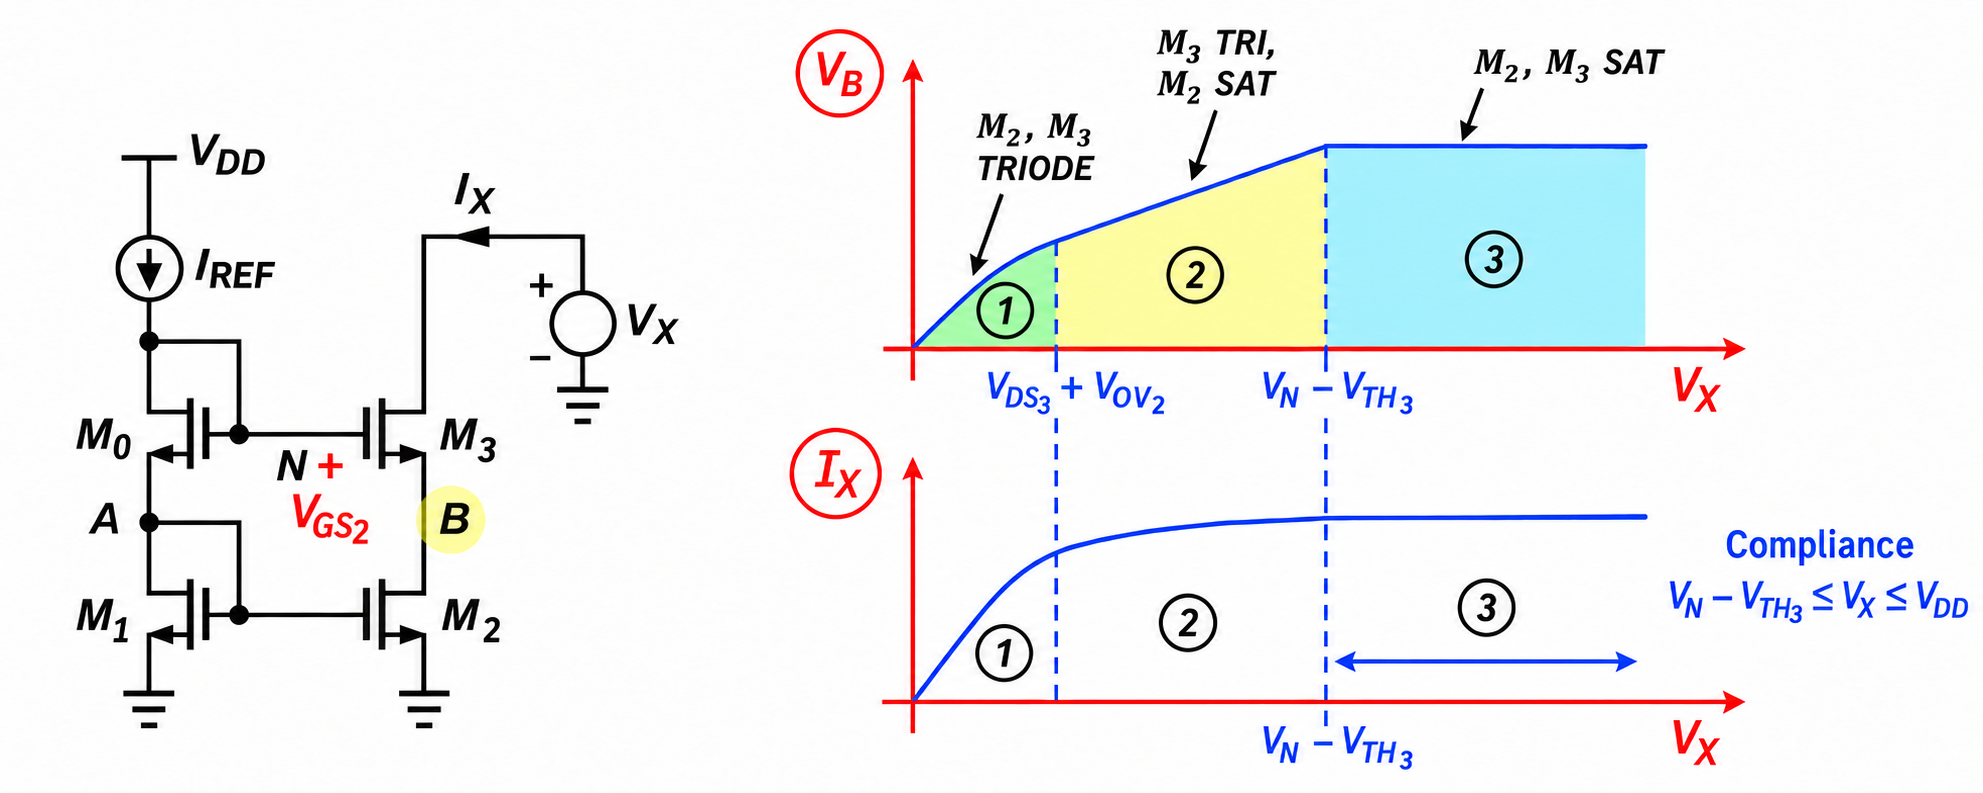
\includegraphics[width=1 \linewidth]{figures/vb-vx-compliance-diagram.png}


\par\noindent\begin{minipage}{\linewidth}
\begin{minipage}[t]{0.48\linewidth}
\vspace{0pt}
\begin{notecircuit}[american, scale=0.55, transform shape]{Conventional Cascode Current Mirror}
    \ctikzset{current arrow scale=24}
    \path[use as bounding box] (-2.4,-1.35) rectangle (4.2,5.55);
    \node[nmos,arrowmos,xscale=-1] (M0) at (0,1.8) {};
    \node[nmos,arrowmos,xscale=-1] (M1) at (0,0) {};
    \node[nmos,arrowmos] (M3) at (2.8,1.8) {};
    \node[nmos,arrowmos] (M2) at (2.8,0) {};
    \node[left] at (-0.45,1.8) {$M_0$};
    \node[left] at (-0.45,0) {$M_1$};
    \node[right] at (3.25,1.8) {$M_3$};
    \node[right] at (3.25,0) {$M_2$};
    \coordinate (ref) at (0,2.65);
    \coordinate (X) at (0,0.9);
    \coordinate (Y) at (2.8,0.9);

    % Retain the highlighted lower reference-gate connection.
    \draw[yellow,opacity=0.4,line width=5pt,line cap=round,line join=round]
        (X) -- (M1.G |- X) -- (M1.G);
    \draw (M0.D) -- (ref) node[circ] {}
        -- (M0.G |- ref) -- (M0.G) node[circ] {} -- (M3.G);
    \node[below,inner sep=2pt] at (1.4,1.8) {$N$};
    \draw (M0.S) -- (X) node[circ] {} node[left] {$X$} -- (M1.D);
    \draw (X) -- (M1.G |- X) -- (M1.G) node[circ] {} -- (M2.G);
    \draw (M3.S) -- (Y) node[right] {$Y$} -- (M2.D);
    \draw (M1.S) -- ++(0,-0.15) node[ground] {};
    \draw (M2.S) -- ++(0,-0.15) node[ground] {};

    \draw[thick] (-0.25,4.25) -- (0.25,4.25);
    \node[right] at (0.3,4.25) {$V_{DD}$};
    \draw[line width=0.3pt] (0,4.25)
        to[I,l=$I_{\mathrm{REF}}$] (ref);
    \node[draw,thick,align=center,font=\sffamily\bfseries,
        minimum width=1.8cm,minimum height=1.3cm,inner sep=4pt]
        (load) at (2.8,4.85) {Analog\\Circuit};
    \node[anchor=north east,inner sep=2pt] at (load.south) {$P$};
    \draw[line width=0.3pt] (load.south)
        to[short,i=$I_{\mathrm{out}}$] (M3.D);
\end{notecircuit}
\end{minipage}\hfill
\begin{minipage}[t]{0.48\linewidth}
\vspace{0pt}
\begin{notecircuit}[american, scale=0.55, transform shape]{High-Swing Cascode Current Mirror}
    \ctikzset{current arrow scale=24}
    \path[use as bounding box] (-2.4,-1.35) rectangle (4.2,5.55);
    \node[nmos,arrowmos] (M0) at (0,1.8) {};
    \node[nmos,arrowmos] (M1) at (0,0) {};
    \node[nmos,arrowmos] (M3) at (2.8,1.8) {};
    \node[nmos,arrowmos] (M2) at (2.8,0) {};
    \node[left] at (-0.15,1.2) {$M_0$};
    \node[left] at (-0.15,-0.65) {$M_1$};
    \node[right] at (3.25,1.8) {$M_3$};
    \node[right] at (3.25,0) {$M_2$};
    \coordinate (X) at (0,2.65);

    % The reference drain drives both lower gates through the outer loop.
    \draw (M0.D) -- (X) node[circ] {} node[right] {$X$}
        -- (-2.35,2.65) -- (-2.35,0) -- (M1.G);
    \draw (M1.G) -- (M2.G);
    \draw (-1.25,1.8) node[circ] {} node[left] {$V_b$}
        -- (M0.G) -- (M3.G);
    \draw (M0.S) -- (M1.D);
    \draw (M3.S) -- (M2.D);
    \draw (M1.S) -- ++(0,-0.15) node[ground] {};
    \draw (M2.S) -- ++(0,-0.15) node[ground] {};

    \draw[thick] (-0.25,4.25) -- (0.25,4.25);
    \node[right] at (0.3,4.25) {$V_{DD}$};
    \draw[line width=0.3pt] (0,4.25)
        to[I,l=$I_{\mathrm{REF}}$] (X);
    \draw[line width=0.3pt] (2.8,3.35)
        to[short,i=$I_{\mathrm{out}}$] (M3.D);
    \node[circle,fill=yellow!35,inner sep=1.5pt] at (0.5,0.9) {$A$};
    \node[circle,fill=yellow!35,inner sep=1.5pt] at (3.3,0.9) {$B$};
\end{notecircuit}
\end{minipage}
\end{minipage}

The purpose of the high-swing cascode CM is keep M2s drain near $V_{OV}$ (the minimum voltage needed to keep it saturated), instead of needlessly holding it at $V_{GS}$. 
This topology is called a \textcolor{red}{"low voltage cascode"}. 
\begin{itemize}
    \item M1 and M2 are still the current copying configuration
    \item M3 and M0 are the bias branches with both of their gates being biased by: $V_b$. But have different source voltages. 
        \begin{itemize}
            \item $V_{GS0} = V_b - V_A$
            \item $V_{GS3} = V_b - V_B$
        \end{itemize}
    \item Conditions for Saturation
        \begin{itemize}
            \item M0: $V_B - V_{TH0} \leq V_X \quad (\mathit{= V_{GS1}})$
            \item M1: $V_{GS1} - V_{TH1} \leq V_A \quad (\mathit{= V_B - V_{GS0}})$
        \end{itemize}
    \item If the cascode devices force: $V_A \approx V_B$ then $V_{DS1} = V_{DS2}$, which gives a very accurate copy.
    \item We choose: $V_b$ such that $V_A = V_B = V_{OV1}$
\end{itemize}
\begin{notetable}{XX}{\textbf{Regular Cascode CM} & \textbf{High-swing Cascode CM}}
    $V_Y \approx V_{GS}$ & $V_Y \approx V_{OV}$ \\
    $V_Y \approx V_{TH} + V_{OV}$ & $V_Y \approx V_{OV}$ \\
    $V_{out,min} = V_{TH} + 2V_{OV}$ & $V_{out, min} = 2V_{OV}$ \\
    More voltage headroom, smaller output swing & less voltage headroom, larger output swing \\
\end{notetable}

\notesection{Current Amplifier}
\par\noindent\begin{minipage}{\linewidth}
\begin{minipage}[t]{0.48\linewidth}
\vspace{0pt}
\begin{notecircuit}[american, scale=0.55, transform shape]{Current Amplifier}
    \ctikzset{current arrow scale=24}
    \path[use as bounding box] (-5.1,-1.9) rectangle (4.5,4.3);
    \node[nmos,arrowmos,xscale=-1] (M1) at (0,0) {};
    \node[nmos,arrowmos] (M2) at (3.3,0) {};
    \node[left] at (-0.45,0) {$M_1$};
    \node[right] at (3.75,0) {$M_2$};
    \coordinate (A) at (0,1.05);
    \coordinate (gate-tie) at (M1.G |- A);
    \draw[yellow,opacity=0.4,line width=5pt,line cap=round,line join=round]
        (A) -- (gate-tie) -- (M1.G);
    \draw (M1.D) -- (A) node[circ] {} node[above right] {$A$}
        -- (gate-tie) -- (M1.G) node[circ] {} -- (M2.G);
    \draw (M1.S) -- ++(0,-0.15) node[ground] {};
    \draw (M2.S) -- ++(0,-0.15) node[ground] {};

    \draw[thick] (-0.25,3.2) -- (0.25,3.2);
    \draw[line width=0.3pt] (0,3.2)
        to[sI,l_=$i_{\mathrm{ref}}$] (A);
    \draw[red,line width=0.3pt] (3.05,3.2) -- (3.55,3.2);
    \draw[color=red] (3.3,3.2) to[R,l=$R_L$] (3.3,1.6);
    \draw[line width=0.3pt] (3.3,1.6)
        to[short,i=$i_{\mathrm{out}}$] (M2.D);

    \node[red] at (0.98,-0.4) {$+$};
    \node[red] at (0.98,-1.0) {$-$};
    \node[red] at (2.32,-0.4) {$+$};
    \node[red] at (2.32,-1.0) {$-$};
    \node[red] at (1.65,-1.5) {$v_{gs1}=v_{gs2}$};

    % M1's small input resistance is an inset annotation, not a third column.
    \draw[blue!70!black,line width=0.3pt,dash pattern=on 2pt off 2pt]
        (0,0.2) ellipse [x radius=1.3,y radius=1.3];
    \draw[blue!70!black,line width=0.3pt,
        -{Latex[length=2pt,width=1.4pt]}]
        (-1.25,0.55) -- (-2.25,0.65);
    \begin{scope}[shift={(-3.5,0.25)},scale=0.65,transform shape,
        color=blue!70!black]
        \node[font=\sffamily\bfseries] at (0,3.0) {$M_1$ equivalent};
        \draw[line width=0.3pt] (0,2.65)
            to[I,l=$i_{\mathrm{ref}}$] (0,1.3);
        \draw (0,1.3) to[R,l=$R_{\mathrm{eq}}$] (0,0)
            node[ground] {};
        \node at (-0.65,1.15) {$+$};
        \node at (-0.65,0.1) {$-$};
        \node[left,inner sep=1pt] at (-0.45,0.65) {$v_{gs1}$};
        \node at (0,-0.75) {$R_{\mathrm{eq}}=\dfrac{1}{g_{m1}}\parallel r_{o1}$};
    \end{scope}
\end{notecircuit}
\end{minipage}\hfill
\begin{minipage}[t]{0.48\linewidth}
\vspace{0pt}
\begin{notecircuit}[american, scale=0.55, transform shape]{Small-Signal Equivalent}
    \ctikzset{current arrow scale=24}
    \path[use as bounding box] (-1.7,-1.9) rectangle (8.9,4.3);
    % Align the source rail, input node, and input source with the amplifier.
    % M1.S is 0.77 below its center; its ground lead adds another 0.15.
    \begin{scope}[shift={(0,-0.92)}]
    \coordinate (A) at (0,1.97);
    \draw[yellow,opacity=0.4,line width=5pt,line cap=round]
        (-0.9,1.97) -- (A);
    \draw (-0.9,1.97) -- (A) node[circ] {} node[above right] {$A$};
    \draw[line width=0.3pt] (-0.8,3.92) node[ground] {}
        -- (-0.8,4.12) -- (0,4.12) to[I,l=$i_{\mathrm{ref}}$] (A);
    \draw (A) to[cI,l=$g_{m1}v_{gs1}$] (0,0) node[ground] {};
    \draw (A) -- (2.4,1.97) to[R,l=$r_{o1}$] (2.4,0);
    \draw (2.4,1.97) -- (3.65,1.97) node[ocirc] {};
    \draw (-0.9,0) -- (7.7,0);
    \draw (3.65,0) node[ocirc] {};
    \node[red] at (-1.15,1.72) {$+$};
    \node[red] at (-1.15,0.2) {$-$};
    \node[red] at (-1.15,0.985) {$v_{gs1}$};
    \node[red] at (3.65,1.72) {$+$};
    \node[red] at (3.65,0.2) {$-$};
    \node[red] at (3.95,0.985) {$v_{gs2}$};

    % M2 has the same gate voltage; its drain remains a separate output node.
    \draw (5.3,1.97) to[cI,l=$g_{m2}v_{gs2}$] (5.3,0)
        node[ground] {};
    \draw[yellow,opacity=0.4,line width=5pt,line cap=round]
        (7.7,1.97) -- (7.7,1.57);
    \draw (5.3,1.97) -- (7.7,1.97) to[R,l=$r_{o2}$] (7.7,0);
    \draw[line width=0.3pt] (7.7,2.52) node[ocirc] {}
        to[short,i=$i_{\mathrm{out}}$] (7.7,1.97);
    \end{scope}
\end{notecircuit}
\end{minipage}
\end{minipage}

\begin{notederivation}{Current Gain, $A_i = \frac{i_{out}}{i_{in}}$ of Current Amplifier}
    & V_{gs1} = V_{gs2} = [i_{ref} - g_{m1} V_{gs1}]\cdot r_{o1} \\
    & V_{gs1} [1 + g_{m1}r_{o1}] = i_{ref}\cdot r_{o1} && \qquad \text{Collecting like terms and isolating for $V_{GS1}$} \\
    & V_{gs1} = i_{ref} \frac{r_{o1}}{1 + g_{m1}r_{o1}} && \qquad \text{Note how: $\frac{r_{o1}}{1 + g_{m1}r_{o1}}$ is equivalent to $R_1$} \\
    & i_{out} = g_{m2} V_{gs2} && \qquad \text{We know that $V_{gs2}$ is equivalent to $V_{gs1}$} \\
    & \therefore i_{out} = g_{m2} \cdot \frac{r_{o1}}{1 + g_{m1}r_{o1}} \cdot i_{ref}
\end{notederivation}

\keyequation{Gain of a Current Amplifier}{A_i = \frac{i_{out}}{i_{ref}} = \frac{g_{m2}r_{o1}}{1 + g_{m1}r_{o1}} \approx \frac{g_{m2}}{g_{m1}}}[
    Since $g_{m1}r_{o1} >> 1$ 
]

\end{document}
